\documentclass{article}


\usepackage{arxiv}

\usepackage[utf8]{inputenc} % allow utf-8 input
\usepackage[T1]{fontenc}    % use 8-bit T1 fonts
\usepackage{hyperref}       % hyperlinks
\usepackage{url}            % simple URL typesetting
\usepackage{booktabs}       % professional-quality tables
\usepackage{amsfonts}       % blackboard math symbols
\usepackage{nicefrac}       % compact symbols for 1/2, etc.
\usepackage{microtype}      % microtypography
\usepackage{lipsum}
\usepackage{fancyhdr}       % header
\usepackage{graphicx}       % graphics
\graphicspath{{figures/}}     % organize your images and other figures under figures/ folder
\usepackage{tikz}
\usepackage{tabularx}
\usepackage{array}
% \usepackage{natbib}
\PassOptionsToPackage{numbers, compress}{natbib}


\newcommand{\halfcircle}{
  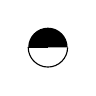
\begin{tikzpicture}[baseline=-0.75ex]
    \fill[black] (0,0) -- (0.25,0) arc (0:180:0.25) -- cycle; % Fill the upper half
    \draw (0,0) -- (-0.25,0) arc (0:180:-0.25); % Draw the border for the lower half
  \end{tikzpicture}
}

%Header
\pagestyle{fancy}
\thispagestyle{empty}
\rhead{ \textit{ }} 

%% Title
% \halfcircle{}
\title{Open-Creator: Bridging Code Interpreter and Skill Library}

\author{
Junmin Gong\(^{*}\) \\
\texttt{gongjunmin@timedomain.ai} \\
Timedomain \\
\and
Sen Wang \(\dagger\) \\
\texttt{sayo@timedomain.ai} \\
Timedomain \\
\and
Wenxiao Zhao \(\dagger\) \\
\texttt{sean.z@timedomain.ai} \\
Timedomain \\
\and
Jing Guo\(\ddagger\) \\
\texttt{joe.g@timedomain.ai} \\
Timedomain \\
}


\begin{document}
\textcolor{red}{\textbf{Note:} The experimental section is currently in progress and will be updated in the subsequent versions.}
\maketitle
\begin{abstract}
AI agents enhanced with tools, particularly code interpreters, hold promising prospects for broad and deep applications. However, existing systems often require reinterpreting problems and generating new codes for similar tasks, rather than reusing previously written and validated functions, leading to inefficiencies in token usage and lack of generalization. In response to these challenges, we introduce \textit{open-creator}, a novel AI agents framework bridging code interpreters and skill libraries. Open-creator is designed to standardize various inputs (including, but not limited to, dialogic problem-solving experiences, code files, and API documentation) into a uniform skill object format. This framework supports local saving, searching, and cloud uploading by users. Adopting a modular strategy, open-creator allows developers and researchers to create, share, and reuse skills without concerns over compatibility or version control. Furthermore, it offers flexibility in modifying, assembling, and disassembling created skills, which is crucial as skills may need updates over time and with changing environments. This mechanism allows AI agents to continually optimize skills based on feedback and new data. Our approach paves the way for more efficient and adaptable AI agent functionalities, contributing to the field's ongoing development. The open-creator code is publicly accessible at: \href{https://github.com/timedomain-tech/open-creator}{https://github.com/timedomain-tech/open-creator}.
\end{abstract}

\section{Introduction}
AI agents engage in complex reasoning by integrating planning ~\cite{wei2022chain, xu2023rewoo, wang2023selfconsistency, yao2023tree}, decision-making, and the utilization of appropriate tools or APIs ~\cite{schick2023toolformer, li2023apibank}. However, these tools are typically predetermined and designed by humans, and the number of available tools is often limited due to the constraints on the input context length of Large Language Models (LLMs). To enhance the versatility of AI agents, a viable approach is to amalgamate the code-generation capabilities of LLMs with code execution functionalities. This integration allows for the flexible writing and execution of code to address specific user needs, embodying the role of Code Interpreters ~\cite{openinterpreter}.

Given that LLMs occasionally generate erroneous codes—leading to low robustness and inability to meet user requirements—recent research has focused on enabling LLMs to auto-correct codes through environmental feedback ~\cite{skreta2023errors, yao2022react, wang2023voyager, song2023llmplanner}. Additionally, there is emphasis on developing sophisticated projects through rational task decomposition and persistent memory. This focus has given rise to a plethora of AI agent frameworks, including MetaGPT ~\cite{hong2023metagpt}, ChatDev ~\cite{qian2023communicative}, GPT-enginger ~\cite{GPTEngineer}, GPT-term ~\cite{GPTeam}, and codeplan ~\cite{bairi2023codeplan}. These studies explore collaborative mechanisms among different roles, introduction of improved environments, enhanced feedback from agents, optimized task decomposition, and various engineering tricks, collectively contributing to the flourishing ecosystem of AI agents in the fields of Computer Science and Software Engineering. A comprehensive literature review in this area has been conducted by Wang et al ~\cite{wang2023survey}.

\begin{table}
\label{tab:learning_approaches}
\begin{tabularx}{\textwidth}{|c|>{\centering\arraybackslash}m{3cm}|>{\centering\arraybackslash}m{4cm}|>{\centering\arraybackslash}m{4cm}|c|}
\hline
 & \textbf{Learning} & \textbf{Outcome} & \textbf{Generalization} & \textbf{Interpretability} \\ \hline
ANN & Parameter Optimization & Weights of NN & Mapping Function & Low \\ \hline
LLM & Instruction Fine-tuning & Instruction-based LLM & In-context Learning Prompt & Medium \\ \hline
Agents & Tool Creation & Skill Library & RAG & High \\ \hline
\end{tabularx}
\centering
\vspace{2mm} % Adjust the space as you need
\caption{Comparison of Different Learning Approaches}
\end{table}

\input{sections/2-related_work}
\begin{figure}[t]
    \centering
    \includegraphics[width=1.1\textwidth]{figures/framework.png}
    \caption{\textbf{The Overview of Open-Creator Framework}}
    \label{fig:framework}
\end{figure}
\input{sections/3-method}
% \section{Experiments}
TODO
% To evaluate the effectiveness of {\framework}, we conduct experiments on two established benchmarks: MATH~\citep{hendrycks2measuring} and TabMWP~\citep{lu2022dynamic}. Though {\framework} benefits various tasks requiring tool creation, we specifically consider these two datasets as representative examples to showcase our framework's strengths. Additionally, we perform experiments on our newly introduced dataset, Creation Challenge, comprising 2K diverse questions that are inadequate to solve using existing tools or code packages. This enables us to further demonstrate the necessity and advantages of the LLM's tool creation ability.

% \begin{figure}[!t]
%     \centering
%     \includegraphics[width=0.49\textwidth]{assets/pic3.pdf}
%     \caption{An example query and its solution provided in the Creation Challenge dataset.} %\chihan{improper indent here. - solved}}
%     \label{fig:creation_challenge}
% \end{figure}

% \begin{table*}[!t]
% \centering
% \small
% \tabcolsep=0.009\linewidth
% \begin{tabular*}{\linewidth}{cccccccccc}
% \toprule
% \textbf{Method}                    & \textbf{Setting} & \textbf{Algebra} & \textbf{\makecell{Counting \& \\ Probability}} & \textbf{Geometry} & \textbf{\makecell{Itmd. \\ Algebra}} & \textbf{\makecell{Number \\ Theory}} & \textbf{\makecell{Pre- \\ Algebra}} & \textbf{\makecell{Pre- \\ Calculus}} & \textbf{\makecell{Average \\ (weighted)}} \\
% \midrule
% \multirow{2}{*}{\textbf{Standard}} 
% & w/o CoT & 25.7 & 25.8 & 22.4 & 13.9 & 18.5 & 40.9 & 21.8 & 25.3 \\
% & w/ CoT   & 50.9 & 36.1 & 24.5 & 17.5 & 23.2 & 58.6 & 16.7 & 37.9 \\
% \midrule
% \multirow{2}{*}{\textbf{\makecell{PoT \\ (w/o Rectify)}}}   
% & w/o CoT & 58.2 & 48.5 & 35.4 & 25.8 & 53.1 & 66.8 & 25.0 & 49.8 \\
% & w/ CoT   & 54.0 & 47.8 & 32.5 & 22.3 & 48.9 & 64.5 & 19.9 & 46.5 \\
% \midrule
% \multirow{2}{*}{\textbf{\makecell{PoT \\ (w/ Rectify)}}}  
% & w/o CoT & 63.8 & 51.9 & 35.9 & 28.6 & 59.2 & 70.0 & 28.2 & 53.9 \\
% & w/ CoT   & 61.4 & 48.8 & 34.6 & 23.7 & 54.5 & 67.6 & 34.6 & 51.2 \\
% \midrule
% \multirow{2}{*}{\textbf{Tool Use}}      
% & w/o CoT & 47.3 & 35.1 & 27.0 & 20.5 & 30.8 & 56.8 & 31.4 & 39.0 \\
% & w/ CoT   & 55.3 & 37.8 & 28.7 & 20.5 & 34.8 & 61.8 & 26.9 & 43.0 \\
% \midrule
% \multirow{3}{*}{\textbf{\makecell{Tool Create \\ (whole)}}}
% & w/o Demo& 58.0 & 53.3 & 34.2 & 21.8 & 55.7 & 63.4 & 33.3 & 49.6 \\
% & w/o CoT & 64.1 & 55.7 & 35.9 & \textbf{42.7} & 61.6 & 69.0 & \textbf{37.2} & 57.2 \\
% & w/ CoT   & 62.7 & 50.9 & 33.8 & 31.4 & 61.4 & 68.7 & 31.4 & 54.0 \\
% \midrule
% \multirow{3}{*}{\textbf{\makecell{{\framework} \\ (ours)}}}
% & w/o Demo& 66.6 & 53.6 & 33.8 & 29.4 & 59.8 & 68.7 & 34.6 & 54.9 \\
% & w/o CoT & \textbf{71.5} & 55.3 & \textbf{41.4} & 41.9 & 60.4 & \textbf{71.7} & 35.3 & \textbf{59.7} \\
% & w/ CoT   & 63.1 & \textbf{58.1} & 34.6 & 35.0 & \textbf{61.8} & 69.7 & 32.1 & 55.7 \\
% \bottomrule
% \end{tabular*}
% \caption{The accuracy (\%) on the test set of MATH dataset leveraging ChatGPT. We report the results of standard QA generation, CoT, PoT, Tool Use, and our {\framework} framework under different settings.}
% \label{tab:MATH_result}%
% \end{table*}

% \subsection{Experimental Setup}
% \paragraph{Base Model.} We select ChatGPT (gpt-3.5-turbo) as the base model for {\framework} due to its exceptional capabilities in code generation, decision making, and logical reasoning. To ensure fairness, we also employ ChatGPT as the base model for all other settings including the chain-of-thought (CoT), program-of-thought (PoT), and tool-use baselines. The maximum generation length for all experiments is set to 512, and a temperature of 0.3 is chosen to encourage deterministic generations while maintaining a certain degree of diversity, particularly during the creation of tools.

% \paragraph{Dataset.} For both MATH and TabMWP datasets, we test {\framework} on all the questions in the test split with numerical value answers (e.g. integer or decimal values). This is due to other answer forms including expressions and fractions are hard to test automatically, and the outputs of programs are prone to give decimal values, which further makes the automatic evaluation complicated. Nevertheless, the test set we apply is able to cover around 80\% of the questions and maintain high diversity, so we regard our results as representative. %\chihan{Can you say ``we follow xxx and do this''?} \cheng{Maybe it's hard to find a former example, but the problems we cover is not manually selected and keeps their diversity.}

% The TabMWP dataset encompasses a wide range of table information and problems of varying difficulty levels, spanning from grade one to grade eight. In the case of the MATH dataset, it encompasses seven domains of math competition problems, including algebra, counting and probability, geometry, intermediate algebra, number theory, pre-algebra, and pre-calculus. Each domain is tested separately, and the weighted average score is computed as the final metric. For the Creation Challenge dataset, we evaluate {\framework} on all 2K data instances and explore the impact of tool creation hints on the LLM's performance.

% \paragraph{Baselines.} We compare {\framework} against three types of baselines to demonstrate its effectiveness:

% \textbf{Standard LLM w/ and w/o CoT}: For Standard LLM with CoT setting, the LLM employs sequential reasoning to solve problems step by step. We also include the baseline Standard LLM without CoT, where the LLM directly generates the answer without employing the reasoning process.

% \textbf{PoT}: The LLM leverages a program to reason through the problem step by step. PoT can be combined with CoT to provide the answer. To ensure a fair comparison specifically focused on the tool creation stage, we also incorporate the rectification module into PoT, making it a stronger baseline.

% \textbf{Tool Use}: The LLM utilizes the WolframAlpha API as a tool for problem-solving. The WolframAlpha API is a general-purpose tool specialized in math calculations. Since all the testing data requires numerical calculations to a certain extent, enabling the LLM to leverage WolframAlpha serves as a fair baseline for LLM's external tool use.

% In addition to these baselines, we introduce another approach by combining the creation stage and decision stage of {\framework} (referred to as \textbf{Tool Create - whole}). In this case, we do not disentangle the abstract tool creation and the concrete decision making. This approach can be seen as a special baseline for ablation studies.

% %\yi{so is the difference between Tool Create - whole and baselines essentially that it adds a rectification step? Or sth else reader may be missing. Maybe I skipped some lines that explained this, my bad (point out to me plz)} \cheng{Tool Create still uses creation stage, but other baselines are not relevant to creation. We set this baseline mainly because we would like to do ablation study on the role of separating creation and decision.}

% \subsection{Creation Challenge}
% %\chihan{The order of Sec4.1 and 4.2 reverses your order of introduction in the previous paragraph. Try to align?}}
% Existing benchmarks are not originally designed to evaluate tool creation, and therefore can not fully
% %\chihan{(too strong. If they fail to showcase, then why would you want to evaluate on them?)}
% showcase the necessity and advantages brought by the LLM's tool creation ability. Therefore, we introduce Creation Challenge to test the LLM's problem-solving skills under new scenarios, without existing tools or code packages that can be directly applied to solve the new problem. Note that although the problems could not be directly solved by existing tools, they could still be leveraged as part of the new tool created if necessary.

% \paragraph{Dataset Construction.} We begin by constructing a seed dataset that involves novel settings and unconventional reasoning processes. Subsequently, we utilize the Text-Davinci-003 model to expand the dataset in an iterative manner. By random sampling from the seed data, we encourage the variety and novelty in the problems and their reasonings.  %\chihan{what kind of new questions are encouraged?}
% Figure~\ref{fig:creation_challenge} illustrates a query and its corresponding solution. Each data entry comprises the problem statement, a standard created tool that can be utilized (including utility, input, output, and realization), a tool-calling decision, and a final answer. % \heng{suggest to change 'sample' to 'a'. 'sample created tool' and 'sample decision' are confusing}

% \paragraph{Evaluation} The components of the standard created tool and the tool-calling decision can serve as valuable hints for the LLM's tool creation and problem-solving. In our experiments, we present the problem to the LLM and assess its tool creation ability with varying levels of hint utilization. The framework's performance is evaluated based on the final answer. We encourage future research to explore the dataset's potential through more flexible usage, further unveiling and testing the capabilities of LLMs.

% \subsection{Experimental Results}

% \paragraph{MATH.} The experimental results on the MATH dataset are presented in Table~\ref{tab:MATH_result}. {\framework} achieves an average accuracy of 59.7\%, surpassing the best performance of the CoT, PoT, and Tool Use methods by 21.8\%, 5.8\%, and 16.7\% respectively. Disentangling the creation stage and decision stage also leads to generally higher accuracy, with an average performance improvement of 2.5\%. We analyze the reasons for the improvement in Section~\ref{analyse_factors}.


% \begin{table}[!t]
% \centering
% \small
% %\tabcolsep=0.015\linewidth
% \begin{tabular}{cccc}
% \toprule
% \textbf{Method} & \textbf{Setting} & \textbf{Accuracy} & \textbf{\makecell{Successful \\ Execution}} \\
% \midrule
% \multirow{2}{*}{\textbf{Standard}} 
% & w/o CoT & 68.2 & 99.1 \\
% & w/ CoT   & 75.2 & 99.3 \\
% \midrule
% \multirow{2}{*}{\textbf{\makecell{PoT \\ (w/o Rectify)}}}   
% & w/o CoT & 80.6 & 98.5 \\
% & w/ CoT   & 80.0 & 91.2 \\
% \midrule
% \multirow{2}{*}{\textbf{\makecell{PoT \\ (w Rectify)}}}  
% & w/o CoT & 81.2 & 99.7 \\
% & w/ CoT   & 87.3 & 100 \\
% \midrule
% \multirow{2}{*}{\textbf{Tool Use}}      
% & w/o CoT & 77.6 & 100 \\
% & w/ CoT   & 79.6 & 100 \\
% \midrule
% \multirow{2}{*}{\textbf{\makecell{Tool Create \\ (whole)}}}
% & w/o CoT & 91.6 & 100 \\
% & w/ CoT   & 93.5 & 99.9 \\
% \midrule
% \multirow{2}{*}{\textbf{\makecell{{\framework} \\ (ours)}}}
% & w/o CoT & 90.5 & 99.7 \\
% & w/ CoT   & \textbf{94.7} & 100 \\
% \bottomrule
% \end{tabular}
% \caption{The accuracy (\%) on the test set of TabMWP dataset leveraging ChatGPT. We report the results of standard QA generation, CoT, PoT, Tool Use, and our {\framework} framework under different settings.}
% \label{tab:TabMWP_result}%
% \end{table}


% \paragraph{TabMWP.} The experimental results on the TabMWP dataset are presented in Table~\ref{tab:TabMWP_result}. For each setting, we measure both the accuracy and the successful execution rate. The successful execution rate indicates whether the LLM provides a final answer within the word limit or the program yields a valid result within the rectification limit. {\framework} achieves an overall accuracy of 94.7\%, outperforming the best settings of CoT, PoT, and Tool Use by 19.5\%, 7.4\%, and 15.1\% respectively. Compared to the standard methods, our framework also achieves a higher successful execution rate. These results highlight the effectiveness of our framework in both text and tabular contexts.


% \begin{table}[!t]
% \centering
% \small
% %\tabcolsep=0.015\linewidth
% \begin{tabular}{cccc}
% \toprule
% \textbf{Method} & \textbf{Setting} & \textbf{Accuracy} & \textbf{\makecell{Successful \\ Execution}} \\
% \midrule
% \multirow{2}{*}{\textbf{Standard}} 
% & w/o CoT & 27.9 & 94.9 \\
% & w/ CoT   & 32.7 & 99.1 \\
% \midrule
% \multirow{2}{*}{\textbf{\makecell{PoT \\ (w/o Rectify)}}} 
% & w/o CoT & 59.2 & 93.5 \\
% & w/ CoT   & 60.7 & 95.7 \\
% \midrule
% \multirow{2}{*}{\textbf{\makecell{PoT \\ (w Rectify)}}} 
% & w/o CoT & 61.1 & 98.3 \\
% & w/ CoT   & 62.0 & 98.9 \\
% \midrule
% \multirow{3}{*}{\textbf{\makecell{Tool Create \\ (whole, \\ w/o CoT)}}}
% & no hint & 64.5 & 99.2 \\
% & utility hint   & 65.8 & 99.3 \\
% & all hint   & 75.3 & 99.5 \\
% \midrule
% \multirow{3}{*}{\textbf{\makecell{{\framework} \\ (ours, \\ w/o CoT)}}}
% & no hint & 63.8 & 98.7 \\
% & utility hint   & 67.2 & 99.1 \\
% & all hint   & \textbf{75.7} & 99.5 \\
% \bottomrule
% \end{tabular}
% \caption{The accuracy (\%) on the Creation Challenge test set leveraging ChatGPT. We report the results of standard QA generation, CoT, PoT, and our {\framework} framework with different levels of hints.}
% \label{tab:CreationChallenge_result}%
% \end{table}


% \paragraph{Creation Challenge.} The experimental results on the Creation Challenge dataset are summarized in Table~\ref{tab:CreationChallenge_result}. In addition to evaluating the LLM's performance under the CoT and PoT settings, we also assess its performance to create tools with varying levels of hints. The "\textit{no hint}" setting represents the standard {\framework} configuration, while the "\textit{utility hint}" provides hints about the utility of the tool, and the "\textit{all hint}" offers additional hints about the possible inputs and outputs of the tool that the LLM may create. Our results demonstrate that even without any hints, {\framework} still outperforms PoT by 1.6\%. As the number of hints provided to the LLM increases, its performance gradually improves, achieving an increase of up to 18.7\% and reaching a high accuracy of 75.5\%. We provide further analysis on the role of hints in Section~\ref{analyse_factors}.

% % \heng{the result analysis needs more insights rather than just repeating numbers} \cheng{The insights are mainly presented in the analysis part. We will further improve the structure in the next edition.}

% \subsection{Results Analysis}
% \paragraph{CoT Incompatible with Codes.} Table~\ref{tab:MATH_result} reveals a consistent decrease in the performance of the LLM on MATH problems when employing the CoT setting, regardless of whether PoT or {\framework} are utilized. In contrast, the opposite trend is observed for TabMWP. We attribute this disparity to the \textbf{inherent incompatibility between natural language reasoning and program-based reasoning when tackling challenging problems}. MATH competition problems, known for their intricate calculations, introduce higher complexity and diversify the possible reasoning paths. This often leads to conflicts between natural language and programming approaches when solving the same problem. When CoT is employed, the LLM tends to incorporate programs that follow natural language reasoning, which potentially compromises the coherence and advantages of programming itself, ultimately resulting in reduced performance. On the other hand, TabMWP also evaluates the model's capacity to extract information from tables, so it involves simpler calculations and a more constrained and straightforward reasoning path. Consequently, this promotes greater consistency between natural language and programming reasoning. Therefore, the application of CoT to such problems enhances performance.

% % Table~\ref{tab:MATH_result} demonstrates that the performance of LLM always declines to some extent on MATH problems under the CoT setting, regardless of whether PoT or Tool Create methods are employed. However, the opposite trend is observed for TabMWP. We attribute this to the \textbf{disparity between natural language thoughts and program thoughts when tackling challenging problems}. MATH competition problems are considerably more complex than TabMWP in terms of calculations. Complexity promotes diverse reasoning paths and is more likely to cause conflicts between natural language and programming methods. When CoT is utilized, the LLM is inclined to generate programs that follow natural language thoughts, which undermines the coherence and advantage of programming itself, and ultimately leading to reduced performance. In contrast, TabMWP also evaluates the model's ability to extract information from tables, resulting in much simpler calculations and a more constrained and straightforward reasoning path. This promotes the consistency between natural language and programming thoughts. Therefore, applying CoT to these questions improves performance.

% \begin{figure*}[!t]
%     \centering
%     \includegraphics[width=0.94\textwidth]{assets/pic4.pdf}
%     \caption{We present three examples from {\framework} and compare the answer given with or without CoT. Challenging problems in MATH cause conflicts between language and program reasonings, while for simpler problems in TabMWP, language and program reasonings complement each other.} % \chihan{a brief sentence explaining the finding.}}
%     \label{fig:CoT_PoT_conflict}
% \end{figure*}

% To illustrate this phenomenon, we present three cases in Figure~\ref{fig:CoT_PoT_conflict}. In the two MATH examples, CoT generates complex tool creation plans that misguide the implementation of tools. Interestingly, without CoT, the adoption of brute-force algorithms and straightforward calculations actually yields higher accuracy. Conversely, for the relatively simpler TabMWP problem, the reasoning path is largely predetermined, making CoT beneficial for tool creation by avoiding unnecessary complexities in problem-solving.

% \begin{figure}[!t]
%     \centering
%     \includegraphics[width=0.49\textwidth]{assets/pic_difficulty.pdf}
%     \caption{Comparison of the accuracy of LLM on baselines and {\framework}, relative to problem difficulty.}
%     \label{fig:difficulty}
% \end{figure}

% \paragraph{Performance Relative to Difficulty.} Figure~\ref{fig:difficulty} illustrates the performance of the LLM in relation to the difficulty levels of the problems. We compare the results of standard methods with and without the application of CoT, as well as the best settings of PoT, Tool Use, and {\framework}. In the case of MATH, the model's performance displays a linear decline as the difficulty level of the questions increases. For TabMWP, the trend was not as pronounced as in MATH, but there is a noticeable drop in accuracy between problems of grades 2 and 3 for both of the standard methods and Tool Use baselines. {\framework} outperforms all the baselines for both tasks and achieves higher accuracy, particularly for difficult problems. This finding provides compelling evidence that \textbf{{\framework} exhibits greater resilience to challenges and more balance when dealing with problems of varying difficulty levels}.

% \begin{figure}[!t]
%     \centering
%     \includegraphics[width=0.49\textwidth]{assets/pic_rectify.pdf}
%     \caption{The improvement of the LLM's performance when the rectification stage is applied for both PoT and {\framework}.}
%     \label{fig:rectification}
% \end{figure}

% \paragraph{Role of Rectification.} The rectification stage is designed to enable the LLM to examine and rectify its own mistakes in case of execution errors, utilizing its intrinsic capacity to detect errors and perform self-correction based on evidence. Figure~\ref{fig:rectification} demonstrates the improvement in the LLM's performance achieved through the application of the rectification stage for both PoT and {\framework}. In this figure, "\textit{Pass@1}" indicates the LLM provides the correct answer directly in the first round without any rectification, while "\textit{Rectify-N}" denotes the LLM retrieves the correct answer within N rounds of rectification. Our results show that \textbf{rectification can increase the accuracy of the LLM by approximately 10\% of the original value}, which proves the necessity and rationality of establishing this stage.


% \paragraph{Influential Factors of Tool Creation.}
% \label{analyse_factors}
% Table~\ref{tab:MATH_result}, Table~\ref{tab:TabMWP_result}, and Table~\ref{tab:CreationChallenge_result} highlight two crucial factors that affect the LLM's performance. (1) \textbf{Separation of Creation and Decision}: the separation of these two stages inherently represents the disentanglement of the LLM's abstract thinking and concrete thinking abilities during problem-solving. This disentanglement can isolate the LLM's distinct reasoning capacities, leading to an improvement in its performance. Our experiments show that the performance of the LLM increases by 4.4\%, 1.3\%, and 0.5\% for MATH, TabMWP, and Creation Challenge, respectively. (2) \textbf{Availability of Hints} In practical scenarios, it is often necessary to provide guidance to LLMs during tool creation in order to better harness their behavior. Therefore, we investigate the role and impacts of hints, and demonstrate through the results of the Creation Challenge that providing more detailed hints can significantly improve the LLM's performance. This is because the utility, input, and output hints can enable the LLM to implement the desired tool much easier with success. Additionally, these hints can eliminate the LLM's uncertainty and reduce any misdirections that may present in CoT or the tool's documentation.

% \input{sections/5-discussions}
% \input{sections/6-conclusion}
\section{Acknowledgements}

We extend our heartfelt appreciation to Killian Lucas, the author of open-interpreter. We are also immensely grateful to the Discord community members, including warjiang, leonidas, AJ Ram, Papillon, minjunes, localman, jofus, Satake, oliveR, piotr, Grindelwald, Nico, MyRealNameIsTim, Pablo Vazquez, and jbexta, for their extensive discussions on the skill library and invaluable feedback. Their collective wisdom greatly enriched our work.

\newpage
%Bibliography
\bibliographystyle{unsrt}
\bibliography{references}  


\end{document}
